%!TEX root = ../phd-thesis-lei-ma.tex

\chapter{\label{chap:dr}Collective Neutrino Oscillations and Dispersion Relations}

Neutrino oscillations in matter background is well defined linear dynamics as we discussed in the preceding chapters. However, the universe provides many other much more exciting labs for neutrino physics. One of such is early supernova explosions, where approximately $10^{58}$ neutrinos are released within seconds~\cite{Bahcall1987}. Such neutrino density would introduce new interaction terms into neutrino oscillations, the self-interaction potential $H_{\nu\nu}$ is comparable or even larger than the matter potential, depending on the region of interest in supernova explosions~\cite{Flowers1976a}. Thus self-interaction between neutrinos is not negligible. Meanwhile, unexpected rich dynamics has be proved to be present with the self-interactions~\cite{Duan2010, Duan2006}. The fact that self-interaction introduces a new characteristic energy scale, new resonances such as matter-neutrino resonance is also possible~\cite{Malkus2014, Vaananen2015, Wu2015}.

In this chapter, I will review the fast modes in neutrino collective oscillations, and clarify the connection between fast modes and dispersion relation proposed by I. Izaguirre et al~\cite{Izaguirre2016a}.



\section{\label{chap:dr-sec:collective}Collective Oscillations}





\subsection{Equation of Motion}

The equation of motion for neutrino oscillations with self-interaction was first derived in \cite{Sigl1993}. For the purpose of the thesis, I will skip the quantum field theory derivations but write it down and clarify some conventions. Without much effort, we know that the equation of motion is the Liouville's equation
\begin{equation}
   i \frac{d}{dt}\rho = [H,\rho]. 
\end{equation}
For the purpose of neutrino oscillations, we always assume they travel with speed of light thus
\begin{equation}
   \frac{d}{dt} = \frac{d}{dr}, 
\end{equation}
where $r$ is the distance travelled by the neutrino. However, in general, what we should have is
\begin{equation}
   \frac{d}{dt} = \partial_t + \mathbf v\cdot \boldsymbol{\nabla}. 
\end{equation}
The Hamiltonian is composed of three different terms,
\begin{equation}
   H = H_{\mathrm v} + H_{\mathrm m} + H_{\nu\nu}, 
\end{equation}
where each term is explicitly written down
\begin{align}
   H_v =& -\frac{1}{2}\beta\eta \omega_0 \sigma_3\\
   H_m =& \frac{1}{2} \sqrt{2}G_F n_e \sigma_3 \\
   H_{\nu\nu} =& \sqrt{2}G_F \int d\omega d\Omega_{\hat v'} n(\omega,\hat v')\beta(\hat v')\rho(\omega,\hat v') (1-\hat v \cdot \hat v').
\end{align}
I use $\eta=\pm 1$ for Normal Hierarchy and Inverted Hierarchy respectively, $\beta=1$ for neutrinos and $\beta=-1$ for antineutrinos. In other words, the vacuum frequency is $\omega_v = \eta \omega_0$. $\beta(\hat v')$ indicates whether the density matrix $\rho(\omega,\hat v')$ is for neutrinos or antineutrinos. If $\rho(\omega,\hat v')$ is for antineutrinos, $\beta(\hat v')=-1$, otherwise $\beta(\hat v')=1$. More explicitly, the vacuum term is
\begin{align*}
   H_v =& \begin{cases}
   -\frac{1}{2}\eta \omega_0 \sigma_3 & \text{for neutrinos}\\
   \frac{1}{2}\eta \omega_0 \sigma_3 & \text{for antineutrinos}
   \end{cases}
\end{align*}
while the neutrino-neutrino interaction Hamiltonian is
\begin{align*}
   H_{\nu\nu} =& \begin{cases}
   \sqrt{2}G_F \int d\omega d\Omega_{\hat v'} n(\omega,\hat v')\rho(\omega,\hat v') (1-\hat v \cdot \hat v') & \text{interacting with neutrinos} \\
   - \sqrt{2}G_F \int d\omega d\Omega_{\hat v'} n(\omega,\hat v')\bar\rho(\omega,\hat v') (1-\hat v \cdot \hat v') &  \text{interacting with antineutrinos}
   \end{cases}
\end{align*}
Please note that in this notion,
\begin{itemize}
    \item $\omega_0$ is meant to be the absolute value of the frequency, since $\eta$ takes care of the signs;
\item The integral in $H_{\nu\nu}$ must take care of both interactions with neutrinos and anti-neutrinos.
\end{itemize}
For simplicity, we define some new quantities.
\begin{itemize}
    \item We define $\lambda$ to measure the matter interactions
    \begin{equation}
        \lambda = \sqrt{2} G_F n_e.
    \end{equation}
\item Angle distribution of number density is defined as
\begin{equation}
    f(\hat v) = \frac{n(\omega,\hat v)}{n_{\mathrm{t}}},
\end{equation}
   where $n_{total}$ is the total number density of neutrinos for all energies. It can also be defined for anti-neutrinos
\begin{equation}
      \bar f(\hat v) = \frac{\bar n(\omega,\hat v)}{\bar n_{\mathrm{t}}},
\end{equation}
where $\bar n_{\mathrm{t}}$ is the total number density of antineutrinos.
In models where neutrinos are emitted from a line, the direction of momentum $\hat v$ depends on one angle, hence $f(\theta)$. With this definition, we know that the number density of neutrinos within an angle $[\theta, \theta + d\theta]$ can be calculated
\begin{equation}
      n_{\mathrm{t}} f(\theta) d\theta.
\end{equation}
Similarly, the the number density of antineutrinos within angle $[\theta,\theta+d\theta]$ is
\begin{equation}
    \bar n_{\mathrm{t}} \bar f(\theta) d\theta.
\end{equation}
\item An asymmetry parameter can be defined to connect the total number density of neutrinos and antineutrinos,
\begin{equation}
    \alpha = \frac{\bar n_{\mathrm{t}} }{n_{\mathrm{t}}}.
\end{equation}

\end{itemize}

With the three definitions we simplify the neutrino self-interactions with matter effect
\begin{align*}
   H_m =& \frac{1}{2} \lambda \sigma_3 \\
   H_{\nu\nu} =& \sqrt{2}G_F n_{\mathrm{t}} \int d\omega d\Omega_{\hat v'} f(\omega,\hat v)\rho(\omega,\hat v') (1-\hat v \cdot \hat v') \\
   & - \sqrt{2}G_F \bar n_{\mathrm{t}} \int d\omega d\Omega_{\hat v'} \bar f(\omega,\hat v)\bar\rho(\omega,\hat v') (1-\hat v \cdot \hat v') \\
   =& \frac{1}{2}\mu \int d\omega d\Omega_{\hat v'} f(\omega, \hat v)\rho(\omega,\hat v') (1-\hat v \cdot \hat v') \\
   & - \frac{1}{2}\alpha \mu \int d\omega d\Omega_{\hat v'} \bar f(\omega, \hat v)\bar\rho(\omega,\hat v') (1-\hat v \cdot \hat v') ,
\end{align*}
where
\begin{equation}
   \mu = 2\sqrt{2} G_F n_{\mathrm{t}}. 
\end{equation}
   



\subsection{Synchronization in Neutrino Oscillations}


With the equation of motion, many aspects of such a system has been explored, such as neutrino bulb model, line model, etc. New dynamics, such as spectral split, synchronizations, matter-neutrino resonances, have been identified~\cite{Duan2006,Malkus2014,Vaananen2015}. Synchronization is one of the most astonishing results which might happen when neutrino number density is high. In this section, I will explain how this is possible.

To grab the flavor of this phenomenon, I use the flavor isospin picture. Flavor isospin was explained in Sec.~\ref{chap:basics-sec:flavor-isospin-pic}. Here we explain another definition of it
\begin{equation}
   \rho = 1 + \frac{1}{2}\vec P \cdot \vec \sigma. 
\end{equation}
For antineutrinos, the flavor isospin is defined as
\begin{equation}
    \bar\rho = 1 - \frac{1}{2} \vec P \cdot \vec \sigma.
\end{equation}
The reason for the negative sign is that we usually reformulate the formula for antineutrinos and define the anti-neutrinos to have negative frequency.

% .. admonition:: Normalization Issue
%   :class: toggle

%   Normalization of polarization vectors are arbitary.

%   When discussing the matter effect only, it's convinient to define it as

%   .. math::
%       \rho =& 1 + \frac{1}{2}\vec P \cdot \vec \sigma\\
%       \bar\rho =& 1 - \frac{1}{2}\vec P \cdot \vec \sigma.

%   However, when it comes to neutrino self-interactions, it's easier to normalize it with :math:`1/n_{\nu}`

%   .. math::
%       \rho =& 1 + \frac{1}{n_\nu}\frac{1}{2}\vec P \cdot \vec \sigma \\
%       \bar\rho =& 1 - \frac{1}{n_\nu}\frac{1}{2}\vec P \cdot \vec \sigma.

%   so that we can write the term

%   .. math::
%       \sqrt{2}G_{\mathrm F} \int dE' (\rho_{E'} - \bar \rho_{E'})

%   to

%   .. math::
%       \sqrt{2}G_{\mathrm F} n_\nu \int dE' \frac{1}{n_\nu}(\rho_{E'} - \bar \rho_{E'}).

%   Then we define

%   .. math::
%       \mu = \sqrt{2}G_{\mathrm F} n_\nu.


With flavor isospin defined, to derive an equation for flavor isospin, we need to decompose the Hamiltonian into vectors. The vacuum and matter part is easy. It's straight forward to write down the vacuum part and matter part of Hamiltonian using three dimensional vectors in flavor isospin space,
\begin{align*}
   \vec H_{\mathrm v} = & \omega_{\mathrm v}\begin{pmatrix}
   -\sin 2\theta_{\mathrm v}\\
   0\\
   \cos 2\theta_{\mathrm v}
   \end{pmatrix}\\
   \vec H_{\mathrm m} = & \begin{pmatrix}
   0\\
   0\\
   -\lambda
   \end{pmatrix}
\end{align*}
But the neutrino coherent scattering term requires some simplifications. For the purpose of the physics picture, we consider isotropic and homogeneous model which leads to
\begin{equation}
   \sqrt{2}G_{\mathrm F} n_\nu \int d\vec p'^3 (1-\vec p \cdot \vec p') (\rho_{\vec p'} - \bar\rho_{\vec p'}) = \sqrt{2}G_{\mathrm F} n_\nu \int dE' \frac{1}{n_\nu}(\rho_{E'} - \bar\rho_{E'}).
   \label{chap:dr-sec:collective-eqn:isotropic-homogeneous-self-interaction}
\end{equation}
We have to define a vector, which is an integral of polarization vector over all energies or frequencies,
\begin{equation}
   \vec D = \int d\omega' \vec P(\omega').
\end{equation}
Expression \ref{chap:dr-sec:collective-eqn:isotropic-homogeneous-self-interaction} becomes $\mu \vec D$, where $\mu = \sqrt{2}G_{\mathrm F} n_\nu$.

For single energy or flavor isospins aligned in the same direction, this vector is in the direction of flavor isospin vector. If flavor isospins were initially prepared in completely random and uniformly distributed directions, $\vec D\sim 0$.

Synchronization occurs when the neutrino number density becomes large. $\vec D$ will wobble around very fast due to the precessions of flavor isospins, but almost stays in one direction. All the spins precess with the same frequency which is determined by $\mu$.

With vacuum contribution $\vec H_{\mathrm v}$ and matter contribution $\vec H_{\mathrm m}$ to the Hamiltonian, we expect $\vec D$ to precess around $\vec H_{\mathrm v} + H_{\mathrm v}$, if the precession frequency of flavor isospins around $\vec D$ is much larger than the precession frequency of $\vec D$ around  $\vec H_{\mathrm v} + H_{\mathrm v}$.





\section{\label{chap:dr-sec:two-beams}Two Beams Model and Linear Stability Analysis}

For nonlinear systems, linear stability analysis comes into play. I will go through the procedure and demonstrate the significance of instabilities and crossing in spectrum. For the sole purpose, I use a simple two-beam line model. The two beams model is simple mathematically, meanwhile reveals the key insights.

In this model, neutrinos are emitted in two different directions from a line which preserves translation symmetry on this line. The emission angles are shown in Fig.~\ref{chap:dr-sec:two-beams-fig:two-beam-line-model}. For convenience of notations, I define a number density distribution function
\begin{equation}
   f(\hat v,\omega)= \frac{n(\hat v,\omega)}{n_t}, 
\end{equation}
where $n_t$ is the total number density of all neutrino emitted, $n(\hat v,\omega)$ is the number density with momentum direction $\hat v$ and energy $\omega$.
We also define
\begin{equation}
   \mu = \sqrt{2}G_F n_t. 
\end{equation}
For two dimensional systems, we can calculate the neutrinos within an angle $[\theta,\theta+d\theta]$
\begin{equation}
   n_t f(\hat v,\omega) d\theta. 
\end{equation}
Similarly we can define the angular distribution for antineutrinos.


\begin{figure}[htbp]
    \centering
    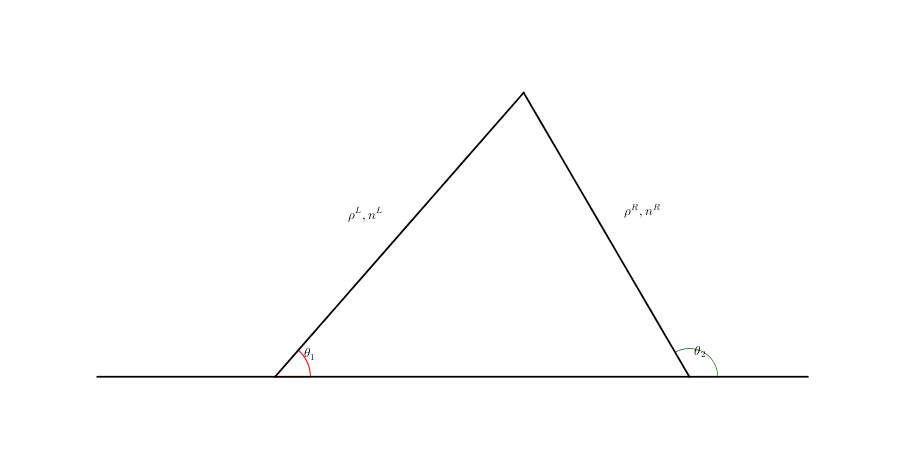
\includegraphics[width=\textwidth]{chapters/assets/dr/two-beam-line-model.png}
    \caption{Geometry of two-beam model to be used in this section. }
    \label{chap:dr-sec:two-beams-fig:two-beam-line-model}
\end{figure}



If all the beams are neutrinos, but with different energies for the left and right beams. The distribution function for beams is delta function. In fact, each beam is just half of the total neutrino number density $n_t$.

The Hamiltonian is a sum of vacuum terms, matter terms, and self-interaction terms,
\begin{equation}
   H= H_v + H_m + H_{\nu\nu}, 
\end{equation}
where
\begin{align}
   H_v =& - \eta \frac{1}{2}\omega \sigma_3 \\
   H_m =& \frac{1}{2}\lambda \sigma_3\\
   H_{\nu\nu}^L =& \frac{1}{2}\mu^R \rho^R (1-\cos(\theta_1-\theta_2))\\
   H_{\nu\nu}^R =& \frac{1}{2}\mu^L \rho^L (1-\cos(\theta_1-\theta_2)).
\end{align}
To linearize the equation of motion, we define the perturbed density matrix as
\begin{equation}
   \rho = \frac{1}{2}\begin{pmatrix}
   1 & \epsilon\\
   \epsilon^* & -1
   \end{pmatrix},
\end{equation}
where we have removed the trace part because it is alway time independent.


The linearized equation of motion becomes
\small\begin{align}
   &i \partial_z \begin{pmatrix}
   \epsilon_1 \\
   \epsilon_2
   \end{pmatrix} =  - i \begin{pmatrix}\cot\theta_1\partial_x & 0 \\
   0 & \cot\theta_2 \partial_x
   \end{pmatrix} \begin{pmatrix}
   \epsilon_1 \\
   \epsilon_2
   \end{pmatrix} \nonumber\\
   &+
   \frac{1}{2}\begin{pmatrix}
   (\lambda+ \mu_2 - \eta \omega_1 - \mu_2 \cos(\theta_1-\theta_2) )/\sin \theta_1 & -\mu_2 (1-\cos(\theta_1-\theta_2)) /\sin \theta_1\\
   -\mu_1 (1- \cos(\theta_1-\theta_2))/\sin\theta_2 & (\lambda + \mu_1 - \eta \omega_2 - \mu_1 \cos(\theta_1-\theta_2) )/\sin\theta_2
   \end{pmatrix}\begin{pmatrix}
   \epsilon_1 \\
   \epsilon_2
   \end{pmatrix},
   \label{chap:dr-sec:two-beams-eqn:line-model-two-beams-all-neutrino-linearized-eom}
\end{align}\normalsize
where
\begin{align*}
   \mu_1 =& \sqrt{2}G_F n_{t,1}\\
   \mu_2 =& \sqrt{2}G_F n_{t,2}. 
\end{align*}
   


\subsection{Left-right Symmetric Emission}


We first consider a simple case, where $\theta_1=\theta_2\equiv\theta$, $\lambda=0$, $\eta=1$, and homogeneous in $x$ direction. For simplicity we define
\begin{align*}
   \mu =& \sqrt{2}G_F (n_1 + n_2)\\
   \mu_i =& \mu \frac{n_i}{n_1+n_2}\equiv \mu f_i \\
   \xi = & 1-\cos(\theta_1-\theta_2)\\
   \omega'_i = & \lambda - \eta\omega_i.
\end{align*}

I am aware that this is not a self-consistent example since $\theta_1=\theta_2$ indicates that $\xi=0$. As we will see, no instability is present in this case. However, we keep the term $\xi$ because we need to analyze the effect of symmetry breaking. This example builds up a formalism.

The equation for perturbations becomes
\begin{equation}
   i\partial_z\begin{pmatrix}
   \epsilon_1 \\
   \epsilon_2
   \end{pmatrix} = \frac{1}{2\sin\theta} \begin{pmatrix}
   \omega'_1 + \mu f_2\xi & -\mu f_2 \xi \\
   -\mu f_1 \xi & \omega'_2 + \mu f_1 \xi
   \end{pmatrix}\begin{pmatrix}
   \epsilon_1 \\
   \epsilon_2
   \end{pmatrix}.
   \label{eqn-linearized-eom-symmetric-eg}
\end{equation}
Since $\mu$ is the most important energy scale in this problem, we scale all energies with it.
\begin{equation}
   i\partial_{\hat z}\begin{pmatrix}
   \epsilon_1 \\
   \epsilon_2
   \end{pmatrix} = \frac{1}{2\sin\theta} \begin{pmatrix}
   \hat\omega'_1 +  f_2\xi & - f_2 \xi \\
   - f_1 \xi & \hat\omega'_2 +  f_1 \xi
   \end{pmatrix}\begin{pmatrix}
   \epsilon_1 \\
   \epsilon_2
   \end{pmatrix},
\end{equation}
where
\begin{align*}
   \partial_{\hat z} =& \frac{d}{\mu dz} \\
   \hat \omega'_i =& \frac{\omega'_i}{\mu}.
\end{align*}


The characteristic equation for this equation is
\begin{equation}
   \left( ( \Omega - \hat\omega'_1 - f_2\xi )(\Omega - \hat\omega'_2-f_1\xi) - f_1 f_2 \xi^2 \right) =0,
   \label{chap:dr-sec:two-beams-eqn:two-beam-line-characteristic-eqn-simple}
\end{equation}
which is simplified to
\begin{equation*}
   (\Omega-\Omega_1)(\Omega-\Omega_2) -f_1f_2\xi^2 = 0,
\end{equation*}
where
\begin{align*}
   \Omega_1 = & \hat\omega'_1 + f_2 \xi\\
   \Omega_2 = & \hat\omega'_2 + f_1 \xi.
\end{align*}
Complete the square
\begin{equation*}
   (\Omega - (\Omega_1 + \Omega_2)/2)^2 = \frac{1}{4}(\Omega_1-\Omega_2) + f_1f_2\xi^2.
\end{equation*}
The solution becomes
\begin{equation}
   \Omega = \frac{1}{2}(\Omega_1+\Omega_2)\pm\sqrt{ (\Omega_1-\Omega_2)^2/4 + f_1f_2\xi^2 }.
\end{equation}
The condition to have positive imaginary part is
\begin{equation*}
   (\Omega_1-\Omega_2)^2 + 4f_1f_2\xi^2 < 0,
\end{equation*}
or
\begin{equation*}
   -2\sqrt{-f_1f_2\xi^2}<\Omega_1-\Omega_2<2\sqrt{-f_1f_2\xi^2},
\end{equation*}
and $f_1f_2\xi^2<0$. Recall the meaning of $f_i$,
\begin{equation*}
   f_i = \frac{n_i}{n_1+n_2}, 
\end{equation*}
instability requires that we have a spectrum crossing, i.e., $n_1$ and $n_2$ have different signs. Plug in the definitions of $\Omega_i$,
\begin{equation*}
   -2\sqrt{-f_1f_2\xi^2}< \eta(- \omega_1 + \omega_2)/\mu + (f_2 - f_1)\xi < 2\sqrt{-f_1f_2\xi^2}.
\end{equation*}
From this we can infer
\begin{itemize}
    \item $f_1f_2$ has to be negative, which means we can NOT have instabilities with only neutrinos or antineutrinos with all the symmetries we assumed. This is crossing.

\item $-\omega_1+\omega_2=0$ will remove the instability. So we have to have both neutrinos and antineutrinos.
\item $f_2-f_1$, $\eta(\omega_2-\omega_1)$, and $\mu$ set limit on each other.
\item $\theta_1=\theta_2\equiv \theta$ removes the instability since it leads to $\xi=0$. The emission has to be asymmetric in this simple two beams model. This is trivial since equal emission angle means the beams are not colliding.
\end{itemize}


% .. admonition:: But why?
%   :class: warning

%   We have these conclusions. But why?

%   What are the roles of

%   1. :math:`f_i`,
%   2. neutrino beam and antineutrino beam,
%   3. hierarchy,
%   4. neutrino number density variations,
%   5. variations of angular distributions of neutrinos,
%   6. variations of energy spectrum of neutrinos.


Another way of understanding this equation is to think of it as the growth of the length of the vector $\vec v = (\epsilon_1,\epsilon_2)^T$. For an arbitrary matrix differential equation of the form
\begin{equation*}
  \partial_z \mathbf v = \mathbf A \mathbf v,  
\end{equation*}
we can always decompose the matrix $\mathbf A$ into symmetric part and skew-symmetric part
\begin{equation*}
  \mathbf A = \frac{1}{2}(\mathbf A + \mathbf A^T) + \frac{1}{2}(\mathbf A - \mathbf A^T) \equiv \mathbf A^+ + \mathbf A^-.
\end{equation*}
We can identify the effect of $f_1-f_2$ but this is not particularly useful since we can not say anything about the eigenvalues of matrix $\mathbf A$ from the eigenvalues of matrix $\mathbf A^+$ and $\mathbf A^-$.



\subsection{Breaking Symmetries}



For a line model, the symmetries we have are
\begin{itemize}
    \item Time translation symmetry;
\item Translation symmetry along the line;
\item Energy spectrum of the beams; One of particular interest is to have different neutrino spheres for different energies which can be investigated using two beam model.
\item Number density of left and right beams;
\item Angle of left and right beams;
\item With and without matter.
\item Similar to the discussion of varying matter potential, symmetries can be broken globally, i.e., distribution as a function of spacetime coordinates.
\end{itemize}

I will discuss some of the symmetries mentioned above.



\subsubsection{Emission Angle Parity Symmetry}

The emission angles change the value of $\xi=1-\cos(\theta_1-\theta_2)$ as well as rescale the quantities by angle dependent factor $1/\sin\theta_i$.

To see the importance of angles, we can redefine some quantities
\begin{align*}
   \omega''_i=& \frac{\omega'_i}{\sin\theta_i}\\
   f''_1=&\frac{f_1}{\sin\theta_2} \\
   f''_2=&\frac{f_2}{\sin\theta_1}.
\end{align*}
The we will reach the same characteristic equation as Eqn. \ref{chap:dr-sec:two-beams-eqn:two-beam-line-characteristic-eqn-simple}. So the angles serves as shift of energy gap and angular distribution.

The region of instability changes in a convoluted way. Given angles we can always write down the expression and find out.
\begin{itemize}
    \item  The criteria of existence of instability doesn't change.
\item  The region of instability changes.
\end{itemize}


\subsubsection{Matter Effect}


Including matter will define vacuum frequencies, $\omega'_i$, which is effectively just a shift of vacuum frequencies. In the symmetric emission case, $\omega'_1-\omega'_2$ is independent of matter effect. But breaking the emission symmetry generates the degeneracy,
\begin{equation}
   \hat\omega''_1-\hat\omega''_2=( \lambda/\sin\theta_1 - \lambda/\sin\theta_2 + \eta(- \omega_1/\sin\theta_1 + \omega_2/\sin\theta_2) )/\mu`.
\end{equation}

We notice that very large matter density shift the region to very small $\mu$.

However, matter effect is not always this simple. Suppose we have different matter potential for different beams, when they collide they would have built a different phase due to matter effect.

The inhomogeneous matter effect has been studied in \cite{Mangano2014}. It can excite high Fourier moments of polarization vector, which makes a lot of sense because it generates fine structure in the x direction. This might be integrated into LESA effect.



\subsubsection{Translation Symmetry}


Translation symmetry is better explained by introducing Fourier transform in x direction. 

For each mode, a term that is proportional to Fourier mode index $m$. It only appears in diagonal elements, thus is effectively a shift of vacuum frequencies, thus energies of neutrinos.

For each Fourier mode
\begin{equation*}
   \begin{pmatrix}
   \epsilon_1 \\
   \epsilon_2
   \end{pmatrix} =  \mathbf Q(\Omega,k) e^{-i(\Omega t- k x)},
\end{equation*}
where we set $\Omega=0$.

First term in RHS of Eqn.~ \ref{chap:dr-sec:two-beams-eqn:line-model-two-beams-all-neutrino-linearized-eom} becomes
\begin{equation*}
   - i \begin{pmatrix}\cot\theta_1\partial_x & 0 \\
   0 & \cot\theta_2 \partial_x
   \end{pmatrix} \begin{pmatrix}
   \epsilon_1 \\
   \epsilon_2
   \end{pmatrix} = k \begin{pmatrix}\cot\theta_1 & 0 \\
   0 & \cot\theta_2
   \end{pmatrix} \begin{pmatrix}
   Q_1 \\
   Q_2
   \end{pmatrix}.
\end{equation*}
We now define $\hat\omega''_i$, so that
\begin{equation*}
   \hat\omega''_{k,i} = \hat \omega''_i + 2\hat k\cot\theta_i,
\end{equation*}
where $\hat k=k/\mu$.

The $k$ term contributes to the difference between $\Omega_{k,i}\equiv \hat\omega''_{k,i}+ f''_i\xi$.

We notice that instability criteria doesn't change. However, the regime of instability changes. We also know that the instability region is determined by
\begin{equation}
   \lvert \Delta\hat\omega''_{12} + 2\hat k (\cot \theta_1 - \cot\theta_2) + \Delta f''_{12}\xi \rvert < \sqrt{-f_1f_2\xi^2},
\end{equation}
where $\Delta \hat \omega''_{12} = \hat\omega''_1-\hat\omega''_2$. The instability region shift from
\begin{equation}
   -\sqrt{-f''_1f''_2\xi^2} -\Delta f''_{12}\xi < (\Delta\omega''_{12} + 2 k(\cot\theta_1-\cot\theta_2))/\mu < \sqrt{-f''_1f''_2\xi^2} -\Delta f''_{12}\xi
\end{equation}
If $\lvert \Delta\omega''_{12} + 2 k(\cot\theta_1-\cot\theta_2) \rvert$ becomes larger, the region of instability is shifted to larger $\mu$, i.e., larger number density.



\subsubsection{Number Density of Emission}


A crossing is required to have instability, i.e., $-f''_1f''_2>0$. Meanwhile the number density on the left and right have little effects on the existence of instability. It shifts the region of instability for $\mu$.


\subsubsection{Energy of Emission}



Different energy of two beams will make sure $-\omega_1 + \omega_2\neq 0$. It has no effects on the criteria but changes the $\mu$ region of instability.


% \subsubsection{Time Translation Symmetry}



% .. admonition:: Time Translational Symmetry
%   :class: warning

%   How about time translational symmetry? I need to write down the equation of motion that is related to time.

%   Two limits are of particular interest.

%   1. Adiabatic limit,
%   2. Superfast time variants.




\subsubsection{General Solutions to Line Model}


For completeness, we solve the general line model, c.f.~Eqn.~\ref{chap:dr-sec:two-beams-eqn:line-model-two-beams-all-neutrino-linearized-eom}. We know that real symmetric matrix has only real eigenvalues, from which we infer that $\mu_1=\mu_2$ and $\theta_1=\theta_2$ removes the instability.
For translation symmetric models, that is $\partial_x\to 0$, we have the eigenvalues
\begin{equation*}
   \Omega = \frac{1}{4}(A\pm B),
\end{equation*}
where
\begin{align*}
   A=& -\eta \omega_1/\sin\theta_1 - \mu_2 /\sin\theta_1 + \eta \omega_2 /\sin\theta_2 + \mu_1 \xi /\sin\theta_2 + \lambda(1/\sin\theta_1 + 1/\sin\theta_2)  \\
   B=& \left(
      -4[(\lambda-\eta\omega_1)(\lambda +\eta\omega_2) + (\lambda (\mu_1-\mu_2) -\eta (\mu_1\omega_1 + \mu_2\omega_2) )\xi ] \sin\theta_1 \sin\theta_2\right. \\
      &\left.+ [(\lambda + \eta\omega_2 + \mu_1\xi) \sin\theta_1 + (\lambda - \eta \omega_1 - \mu_2\xi) \sin\theta_2 ]^2
   \right)^{1/2}/(\sin\theta_1\sin\theta_2)\\
   \xi=&1-\cos(\theta_1-\theta_2).
\end{align*}


For antineutrinos, I only need to change $\mu_i\to -\bar\mu_i$ and $\omega_i\to -\bar\omega_i$, where $\bar\mu=\sqrt{2}G_F \bar n_t$, so that the equation becomes
\small\begin{align*}
  &i \partial_z \begin{pmatrix}
  \epsilon_1 \\
  \epsilon_2
  \end{pmatrix} =  - i \begin{pmatrix}\cot\theta_1\partial_x & 0 \\
  0 & \cot\theta_2 \partial_x
  \end{pmatrix} \begin{pmatrix}
  \epsilon_1 \\
  \epsilon_2
  \end{pmatrix} \\
  &+
  \frac{1}{2}\begin{pmatrix}
  (\lambda-\bar\mu_2 + \eta \bar\omega_1 + \bar\mu_2 \cos(\theta_1-\theta_2) )/\sin \theta_1 & \bar\mu_2 (1-\cos(\theta_1-\theta_2)) /\sin \theta_1 \\
  \bar\mu_1 (1- \cos(\theta_1-\theta_2))/\sin\theta_2 & (\lambda -\bar\mu_1 + \eta \bar\omega_2 +\bar\mu_1 \cos(\theta_1-\theta_2) )/\sin\theta_2
  \end{pmatrix}\begin{pmatrix}
  \epsilon_1 \\
  \epsilon_2
  \end{pmatrix}
\end{align*}\normalsize

Assume that the left beam is neutrino beam and the right beam is antineutrno beam. The linearized equation of motion becomes
\small
\begin{align*}
  &i\partial_z \begin{pmatrix}
  \epsilon_1 \\
  \epsilon_2
  \end{pmatrix} =  -i\begin{pmatrix}
  \cot\theta_1 \partial_x & 0 \\
  0 & \cot\theta_2 \partial_x
  \end{pmatrix}\begin{pmatrix}
  \epsilon_1 \\
  \epsilon_2
  \end{pmatrix} \\
  &+ \frac{1}{2}\begin{pmatrix}
  (\lambda - \bar\mu - 2\eta \omega_1 + \bar\mu \cos(\theta_1-\theta_2) )/\sin\theta_1 & \bar\mu (1-\cos(\theta_1-\theta_2))/\sin\theta_1 \\
  -\mu(1-\cos(\theta_1-\theta_2))/\sin\theta_2 & (\lambda + \mu + \eta \omega_2 - \mu \cos(\theta_1-\theta_2) )/\sin\theta_2
  \end{pmatrix}\begin{pmatrix}
  \epsilon_1 \\
  \epsilon_2
  \end{pmatrix}
\end{align*}
\normalsize


% Numerical Calculations
% ~~~~~~~~~~~~~~~~~~~~~~~~~~~~~~


% We assume the two beams have different energy, as indicated by :math:`\omega_1` and :math:`\omega_2` in Eq. \ref{chap:dr-sec:two-beams-eqn:line-model-two-beams-all-neutrino-linearized-eom}


% For numerical calcualtions, we scale quantities using :math:`\mu`.

% With symmetric angles for the two beams, I didn't find instabilities. However, :math:`\theta_1\neq \theta_2` leads to instabilities in IH, which is consistant with our expections.



% For NH:


% .. image:: assets/some-clarifications/allneutrinos/line-two-beam-eta-1-lambda-0-mu-10-alpha-0.5-theta1-pi-div-3-theta2-pi-div-6.png
%   :width: 31%
% .. image:: assets/some-clarifications/allneutrinos/line-two-beam-eta-1-lambda-0-mu-10-alpha-1.-theta1-pi-div-3-theta2-pi-div-6.png
%   :width: 31%
% .. image:: assets/some-clarifications/allneutrinos/line-two-beam-eta-1-lambda-0-mu-10-alpha-1.5-theta1-pi-div-3-theta2-pi-div-6.png
%   :width: 31%

% .. image:: assets/some-clarifications/allneutrinos/line-two-beam-eta-1-lambda-0-mu-10-alpha-0.5-theta1-pi-div-6-theta2-pi-div-3.png
%   :width: 31%
% .. image:: assets/some-clarifications/allneutrinos/line-two-beam-eta-1-lambda-0-mu-10-alpha-1.-theta1-pi-div-6-theta2-pi-div-3.png
%   :width: 31%
% .. image:: assets/some-clarifications/allneutrinos/line-two-beam-eta-1-lambda-0-mu-10-alpha-1.5-theta1-pi-div-6-theta2-pi-div-3.png
%   :width: 31%

% .. image:: assets/some-clarifications/allneutrinos/line-two-beam-eta-1-lambda-0-mu-10-alpha-0.5-theta1-pi-div-3-theta2-pi-div-3.png
%   :width: 31%
% .. image:: assets/some-clarifications/allneutrinos/line-two-beam-eta-1-lambda-0-mu-10-alpha-1.-theta1-pi-div-3-theta2-pi-div-3.png
%   :width: 31%
% .. image:: assets/some-clarifications/allneutrinos/line-two-beam-eta-1-lambda-0-mu-10-alpha-1.5-theta1-pi-div-3-theta2-pi-div-3.png
%   :width: 31%



% Non-local Symmetry Breaking
% -----------------------------









\section{\label{chap:dr-sec:fast-mode}Fast Mode}


In a paper by Chakraborty et al~\cite{Chakraborty2016}, they showed that neutrino flavor instabilities can grow with a rate that is proportional to the neutrino density, which has much faster oscillation frequencies than vacuum oscillations. For such a fast growth to happen, the author considered head on colliding neutrino beams. The derivation is much similar to what has been shown in the previous section.

As an estimation, the frequencies of vacuum oscillation is
\begin{align*}
   \omega_{\mathrm v} =& \frac{\Delta m^2}{2E} \\ \sim& 6.3\times 10^{-3} \mathrm{m}^{-1}  \frac{\Delta m^2_{32}}{2.5\times 10^{-3} \mathrm{eV}^2 } \frac{1MeV}{E} \\
   \sim & 1.90\times 10^{-4}  \mathrm{m}^{-1}  \frac{\delta m^2}{7.5\times 10^{-5}\mathrm{eV}^2} \frac{1\mathrm{MeV}}{E},
\end{align*}
where $E$ is the neutrino energy. The corresponding oscillation wavelength is simply give by
\begin{align*}
   \lambda_{12} = & 2\pi/\omega_{12} \sim 1 \mathrm{km}\\
   \lambda_{32} = & 2\pi/\omega_{32} \sim 33.1 \mathrm{km}.
\end{align*}
The fast modes instability grows with a rate proportional to the neutrino potential $\mu=\sqrt{2}G_F n_\nu$, which is very large in dense neutrino media. A large growth rate indicates a faster flavor transformation than vacuum oscillations.




% \subsection{\label{chap:dr-sec:fast-mode-subsec:introduction}Introduction}

% (Should talk about some very very basic backgrounds like the applications and why it is important.)





\subsection{\label{chap:dr-sec:fast-mode-subsec:dr}Dispersion Relation of Neutrino Flavor Conversion}

We consider two-flavor scenario ($\nu_{\mathrm e}$ and $\nu_{\mathrm x}$) of neutrino oscillations. We also assume that all neutrinos and antineutrinos are emitted as electron flavor. The flavor evolution of neutrino ensemble depends on flavor density matrices of neutrinos $\rho$ and antineutrinos $\bar\rho$ with energy $E$, direction of velocity $\hat{\mathbf v}$,
\begin{equation}
\ii (\partial_t + \mathbf v\cdot \mathbf{\nabla}) \rho = \left[H, \rho_n \right],
\label{eqn-liouville-eqn}
\end{equation}
where $H$ is the Hamiltonian for neutrino oscillations. In the context, Hamiltonian depends on three different contributions from vacuum oscillations $H_{\mathrm v}$, interactions with matter $H_{\mathrm m}$, and interactions with neutrinos themselves $H_{\nu\nu}$. In this work, we ignore vacuum and matter terms since the concentration is on fast neutrino oscillations, which would occur even without neutrino mass differences \cite{Chakraborty2016,Dasgupta2017}. In order to calculate the neutrino self-interaction term $H_{\nu\nu}$, the distribution of neutrinos (antineutrinos) $f_{\nu_{\mathrm e}(\bar \nu_{\mathrm e})}(\hat{\mathbf v}, E)$ and $f_{\nu_{\mathrm x}(\bar \nu_{\mathrm x})}(\hat{\mathbf v}, E)$ is required, where $E$ is the energy of neutrinos (antineutrinos). We have
\begin{equation}
H_{\nu\nu} = \sqrt{2} G_{\mathrm F} \iint \frac{\mathrm d \cos\theta' \mathrm d\phi'}{4\pi} v^\mu v'_\mu \int \frac{E'^2 \mathrm d E'}{2\pi^2} \left( (f_{\nu_{\mathrm e}}' - f_{\nu_{\mathrm x}}' )\rho' -  (f_{\bar\nu_{\mathrm e}}' - f_{\bar\nu_{\mathrm x}}' ) \bar\rho' \right),
\end{equation}
where $v^\mu = ( 1, \sin\theta\cos\phi, \sin\theta\sin\phi, \cos\theta )^{\mathrm T}$ is the four velocity of (anti)neutrinos in our spherical coordinate system. Without vacuum contribution, the equation of motion for antineutrinos has the same form \cite{Duan2010}.

We follow the same assumption in reference \cite{Izaguirre2016a} that the the distribution of $\nu_x$ and $\bar\nu_x$ are the same, namely $ f_{\nu_{\mathrm x}}(\hat{\mathbf v},E)  - f_{\bar\nu_{\mathrm x}}(\hat{\mathbf v},E)=0$. In addition, we have the same definition of electron lepton number (ELN) of neutrinos travelling in direction $\hat{\mathbf v}$ \cite{Izaguirre2016a},
\begin{equation}
G(\hat{\mathbf v}) =  \sqrt{2}G_{\mathrm F} \int \frac{E'^2 \mathrm d E'}{2\pi^2} ( f_{\nu_{\mathrm e}}(\cos\theta',\phi',E')  - f_{\bar\nu_{\mathrm e}}(\cos\theta',\phi',E')  ).
\end{equation}
To perform linear stability analysis, we assume that the density matrix has the form
\begin{equation}
\rho = \bar \rho = \begin{pmatrix}
1 & \epsilon \\
\epsilon^* & 0
\end{pmatrix},
\end{equation}
where $\lvert \epsilon \rvert \ll 1$. As a result, the linearized equations of motion depends only on $G(\hat{\mathbf v})$ and $\hat{\mathbf v}$. We also assume that all neutrinos and antineutrinos undergo the same behavior in linear regime, $\epsilon = \tilde\epsilon e^{-\ii (\Omega t - \mathbf K\cdot \mathbf x)}$. Izaguirre, Raffelt, and Tamborra defined the polarization tensor \cite{Izaguirre2016a},
\begin{equation}
\Pi^\mu_{\phantom{\mu}\nu} = 1 + \int \frac{d\Omega}{4\pi} G(\theta,\phi) \frac{v^\mu v_\nu}{\omega- k \hat{\mathbf k}\cdot \hat{\mathbf v} },
\end{equation}
which defines the dispersion relation $\Pi^\mu_{\phantom{\mu}\nu} a^\nu = 0$, with $a^\nu = \int \frac{d\cos\theta' d\phi'}{4\pi} G(\hat{\mathbf v}') v^\nu \tilde\epsilon$. We find the nontrivial solutions by setting \cite{Izaguirre2016a},
\begin{equation}
\operatorname{det}\left( \Pi^\mu_{\phantom{\mu}\nu} \right) = 0.
\label{eqn-dr-determinant-equation}
\end{equation}


For simplicity, we consider axial symmetric neutrino emission so that Eq. \eqref{eqn-dr-determinant-equation} becomes
\begin{align}
&\det \left( \omega \mathrm{I} + \frac{1}{2}
\begin{pmatrix}
   I_0 & 0 & 0 & -I_1 \\
   0 & -\frac{1}{2} (I_0 - I_2) & 0 & 0 \\
   0 & 0 & -\frac{1}{2} (I_0 - I_2) & 0 \\
   I_1 & 0 & 0 & -I_2
\end{pmatrix}\right) \nonumber\\
&=0,
\label{eqn-det-polarization-tensor-axial}
\end{align}
where $\mathbf I$ is the rank 4 identity matrix and
\begin{equation}
   I_m =\int_{-1}^{1} d u G(u) \frac{u^m}{1 -  \left(\lvert k\rvert /\omega\right) u }.
\end{equation}
where we define $u=\cos\theta$. Eq. \eqref{eqn-det-polarization-tensor-axial} is equivalent to the result in reference \cite{Raffelt2013}. $\lvert k \rvert /\omega$ is defined as the refractive index $n$ of the flavor wave. For spectrum $G(u)$ without zero values, the forbidden region is given by $1 -  \left(\lvert k\rvert /\omega\right) u\leq 0$.

The dispersion relations can be categorized into two different types by symmetries. To incorporate azimuthal symmetry, we define solutions related to the first and second element of $a^\nu$ ($\nu=1,2$) to be multi-azimuthal angle (MAA) solutions since they are the only solutions that depend on azimuthal angle $\phi$. The other solutions which are related to $\nu=0,3$ are defined to be the multi-zenith angle (MZA) solutions. The MAA solution is related to symmetry breaking in azimuthal angle only, which is determined by
\begin{equation}
   \omega = \frac{1}{4}(I_0 - I_2).
   \label{eqn-maa}
\end{equation}
Similarly, the MZA solution is related to symmetry breaking in both azimuthal angle and zenith angle, which is
\begin{equation}
\omega = - \frac{1}{4} \left( I_0 - I_2 \pm \sqrt{ (I_0 + I_2 - 2 I_1) (I_0 + I_2 + 2 I_1) } \right).
\label{eqn-mza}
\end{equation}
We denote the solution associated with $+$ sign in Eq. \eqref{eqn-mza} as MZA+, while the solution assocated with $-$ sign as MZA-. The two solutions are connected to each other in dispersion relations. In general, it doesn't provide physical insights to distingush the two branches of solutions since they are simply two branches of the solution.

The solutions to Eq. \eqref{eqn-maa} and Eq. \eqref{eqn-mza} are dispersion relations $D(\omega,\mathbf k)$ for a chosen direction of $\hat{\mathbf k} = \hat{\mathbf z}$ with axial symmetric neutrino emission.



%%%%%%%%%%%%%%%%%
%% To BE Added
%%%%%%%%%%%%%%%%
% {\color{red}{\bf HAVE TO EXPLAIN THE IDEA OF GAP AND INSTABILITY HERE. Maybe Later?}}






\subsection{\label{chap:dr-sec:fast-mode-subsec:instabilities-and-gaps}Instabilities and Gaps}

In reference \cite{Izaguirre2016a}, the authors relate gaps in dispersion relation to instabilities of neutrino oscillations. In this section, we review the idea of correspondence between gaps and instabilities first. Then we show that this relation is not a solid theory that can be generalized to all cases.

We continue the discussion of axial symmetric neutrino emissions but with discretized zenith angles $\theta$ thus discretized $u$. Hence the ELN is independent of azimuth angle $\phi$. For neutrino emission with $2$ zenith angles, the ELN spectrum is
\begin{equation}
G(u)= \sum_{i=1}^2 g_i \delta(u - u_i).
\end{equation}

The MAA solution becomes an equation of hypobola for $\omega$ and $k$, which has asymptotes $\omega = k u_i$ for $i=1,2$. Meanwhile, hyperbola equation has two solutions of $\omega$ ($k$) for any given real $k$ ($\omega$). The solutions are either real which indicates stable solutions or complex which indicates exponential growth or decrease in linear regime. On the other hand, non-existence of real solutions of $\omega$ ($k$) for given real $k$ ($\omega$) is equivalent to gap in dispersion relation. Thus the equivalence of gap and instabilities is guaranteed in neutrino emission with two-zenith-angle emission. The numerical calculations is normalized using the maximium value in spectrum which is a convention we follow for all discrete emission calculations. Unit for $\omega$ and $k$ can be determined once the exact spectrum is determined. Upper panels of Fig. \ref{fig-dr-db} is reproduction of left panels of Fig. 1 in reference \cite{Izaguirre2016a}. The dispersion relation is shown as black lines. The real part $\omega_{\mathrm R}$ is shown as red solid lines. $\omega_{\mathrm R} \pm \omega_{\mathrm I}$ are shown are red dashed lines, where $\omega_{\mathrm I}$ is the imaginary part of $\omega$.



\begin{figure}[!htb]
\minipage{0.49\textwidth}
  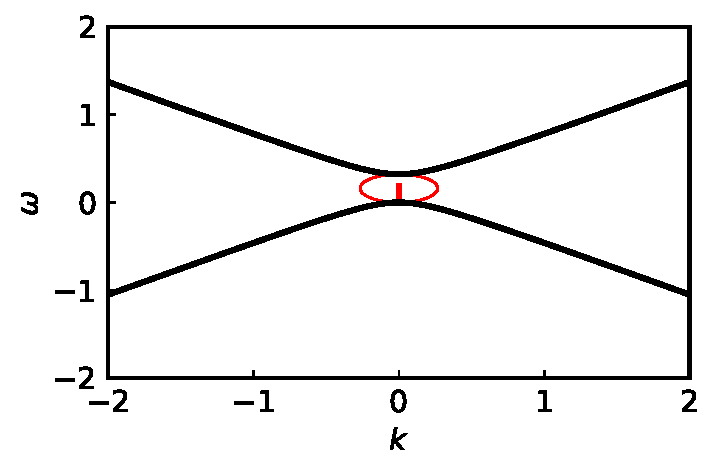
\includegraphics[width=\linewidth]{chapters/assets/dr/spectDBWC1DRDBMAAPltBlob.pdf}
\endminipage\hfill
\minipage{0.49\textwidth}
  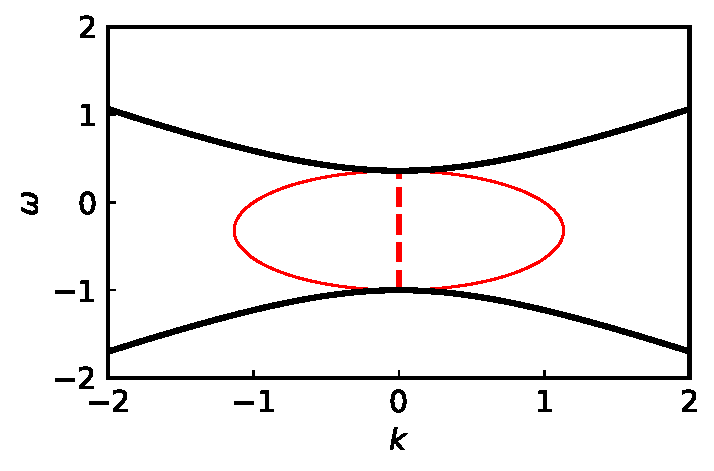
\includegraphics[width=\linewidth]{chapters/assets/dr/spectDBWC1DRDBMZAPltBlob.pdf}
\endminipage\hfill
\newline
\minipage{0.49\textwidth}
  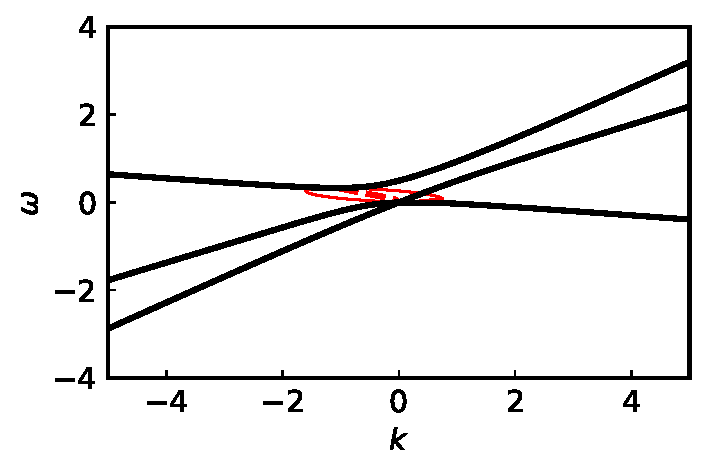
\includegraphics[width=\linewidth]{chapters/assets/dr/spectDB3WC4DRDBMAAPltBlob.pdf}
\endminipage\hfill
\minipage{0.49\textwidth}
  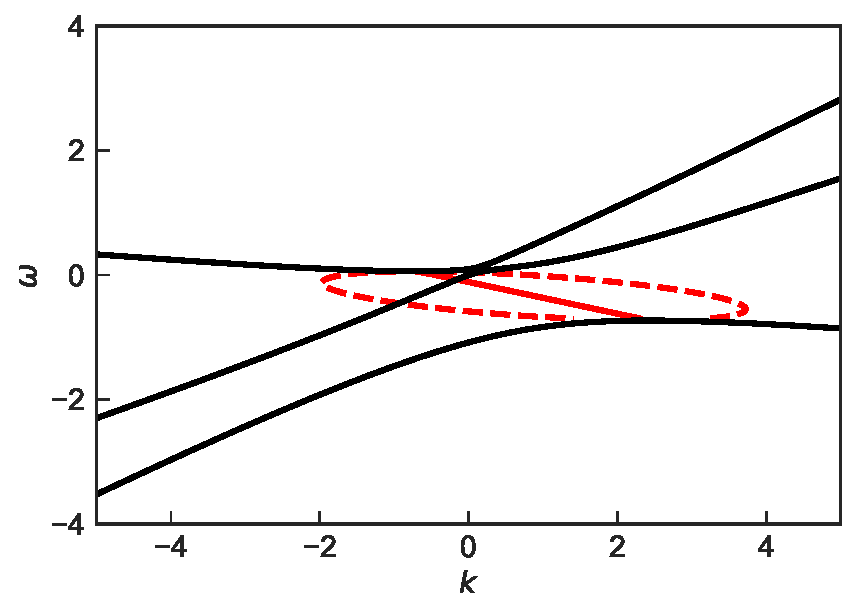
\includegraphics[width=\linewidth]{chapters/assets/dr/spectDB3WC4DRDBMZAPltBlob.pdf}
\endminipage\hfill
\caption{Dispersion relation and instabilities of two zenith angles spectrum (upper panels) and three zenith angles spectrum (lower panels). The black lines are the dispersion relations and the colored dots are examples of complex $\omega$ for real $k$. The left panels are the dispersion relation and linear stability analysis of MAA solutions while the right panels are for MZA solutions.}
\label{fig-dr-db}
\end{figure}



In core collapse supernova and neutron star mergers, neutrino emission is not in discrete zenith angles. More realistic models involve continuous zenith angle ELN spectra. In the case that the smooth and continuous ELN spectrum has no crossing, gap indeed indicates instabilities, as shown in reference \cite{Izaguirre2016a}. In this section we prove that the instabilities in MAA, MZA+, or MZA- solution can only appear in either region $\omega\leq 0$ or region $\omega \geq 0$. As it suggests, the instability regions propagate only between the dispersion relation curves and the axis $\omega=0$. We reproduced the calculation in reference \cite{Izaguirre2016a} using the same Garching core-collapse supernova data set \cite{garching-ccsn-data}. The spectrum shown in the left panel of Fig. \ref{fig-garching} is polynomial fitting of the Garching 1D supernova simulation data. On the right of Fig. \ref{fig-garching}, the dispersion relation for MAA (MZA) solution is shown as red (green, blue) solid lines. Instabilities associated with MAA (MZA) solution is shown as light red (light green, light blue) blobs. The two branches of MZA solutions appear at the top half (MZA+) and lower half (MZA-). The result shows that instabilities occur either in region $\omega>0$ or region $\omega<0$ and with limits set the dispersion relation. We will prove that the instabilities appear between the dispersion relation and the axis $\omega=0$.






\begin{figure}
   \minipage{0.49\textwidth}
     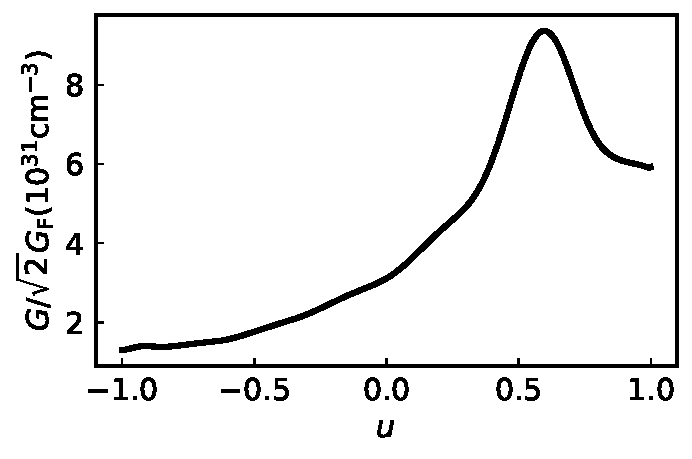
\includegraphics[width=\linewidth]{chapters/assets/dr/spectGarchingPlt.pdf}
   \endminipage\hfill
   \minipage{0.49\textwidth}
   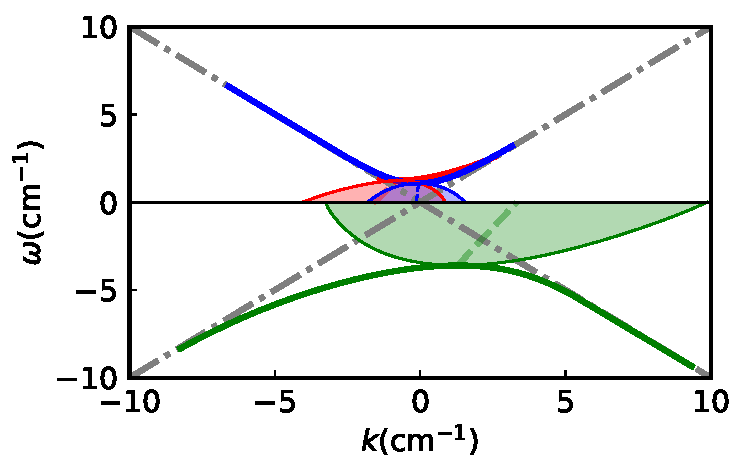
\includegraphics[width=\linewidth]{chapters/assets/dr/spectGarchingDRLSAPltBlob.pdf}
   \endminipage\hfill
   \caption{Dispersion relation and linear stability analysis (right panel) for a spectrum constructed from Garching 1D simulation data (left panel). Solid red line is dispersion relation for MAA solution while blue and green lines are for MZA solutions. Light red (green and green) blob is instability for MAA (MZA) solution.
    }
   \label{fig-garching}
\end{figure}




% \subsection{\label{sec-omega-to-zero}Instabilities at $\omega\to 0$}

Suppose we are looking for complex solutions for given real omega as in Fig. \ref{fig-garching}, MAA solution Eq. \eqref{eqn-maa} is rewritten as a function $k(\omega/k)$. More explicitly, we have to solve the integral function to find out $k$ for real $\omega$,
\begin{equation}
   k = \frac{1}{4} \int \mathrm du G(u) \frac{ 1 - u^2 }{ \omega/k - u }.
   \label{eqn-k-omega-relation}
\end{equation}
To investigate how instabilities developed around the horizental axies, we solve Eq. \eqref{eqn-k-omega-relation} in the limit $\omega\to 0$. For complex $k$, the integral can be decomposed into the principal value $\operatorname{Re}(k)$ and imaginary part $\operatorname{Im}(k)$ using Sokhotski–Plemelj theorem,
\begin{subequations}
\begin{align}
\operatorname{Re}(k) =& \frac{1}{4}\left(  \mathcal{P} \int \mathrm d u G(u) \frac{ 1 - u^2 }{ - u }  \right)\label{eqn-re-k-arbitrary-spectrum} \\
\operatorname{Im}(k) =&  \frac{\pi}{4}G(0) \operatorname{Sign}\left( \omega \right) \operatorname{Sign}\left(  \operatorname{Im}(k)  \right).
\label{eqn-im-k-arbitrary-spectrum}
\end{align}
\end{subequations}
Assuming no crossing is found in sepctrum $G(u)$ at $u=0$, Eq. \eqref{eqn-im-k-arbitrary-spectrum} shows that $\omega$ must have the same sign as $G(0)$ if we find nonzero imaginary part in $k$. We conclude that instabilities can only grow either in the upper plane $\omega>0$ or lower plane $\omega<0$. What's more, the value of $k$ at limit $\omega\to 0$ can be solved out of Eq. \eqref{eqn-re-k-arbitrary-spectrum} and Eq. \eqref{eqn-im-k-arbitrary-spectrum}. For instabilities the imaginary part of $k$ tells us the growth rate is,
\begin{equation}
   \lvert \operatorname{Im}(k) \rvert  =  \frac{\pi}{4}\lvert G(0)\rvert .
\end{equation}
Similar result is obtained for MZA solutions,
\begin{align}
&\left(4\operatorname{Re}(k) - \mathcal P \int \frac{G(u)}{u} \mathrm d u + U_1 \right)^2  - \left( \operatorname{Sign}(\omega \operatorname{Im}(k) )\pi G(0) +4 \operatorname{Im}(k) \right)^2 \\
% =&\left( \mathcal P \int \frac{G(u)}{u} \mathrm d u + U_1 \right)^2 -1 - 4 U_0^2  \\
% &\left( 4 \operatorname{Re}(k) - \mathcal P \int \frac{G(u)}{u} \mathrm d u + U_1 \right) \left( \pi \operatorname{Sign}(\omega \operatorname{Im}(k) ) G(0) + 4 \operatorname{Im}(k) \right) \\
=& - \left( \mathcal P \int \frac{G(u)}{u} \mathrm du + U_1 \right) \pi \operatorname{Sign}(\omega \operatorname{Im}(k) ) G(0),
\end{align}
where $U_m = \int G(u) u^m \mathrm du$ and all the integrals are over all the sepctrum. The equations are quadratic in both $\operatorname{Re}(k)$ and $\operatorname{Im}(k)$ so the real solutions can be calculated and verified with linear stability analysis. The imaginary part $\operatorname{Im}(k)$
\begin{equation}
   \operatorname{Im}(k) = - \frac{1}{4} \pi G(0) \operatorname{Sign}(\omega \operatorname{Im}(k) ) \left(  1 \pm \frac{ \mathscr P \int \frac{G(u)}{u} du + \int G(u) u du }{ 4 \operatorname{Re}(k) - \mathscr P \int \frac{G(u)}{u} du + \int G(u) u du }  \right)
\end{equation}
determines that the two different solutions are either in the region $\omega>0$ or in the region $\omega<0$ which corresponds to MZA+ and MZA- solutions. The instabilities in the two regions are not continuous at $\omega=0$.



\subsection{\label{chap:dr-sec:fast-mode-subsec:instability-to-gap}Instabilities Do Not Always Show Up as Gap}

Even though the concept of gap leads to instabilities works well for the models in \ref{chap:dr-sec:fast-mode-subsec:instabilities-and-gaps}, it can not be generalized to arbitrary number of emission angles nor to continuous spectra with crossings. As an example, we perform linear stability analysis of the three zenith angles emission configuration which is determined by a cubic function both in $\omega$ and $k$. Three solutions of $k(\omega)$ for given real $\omega(k)$  are expected. As long as real solutions disappear, complex solutions emerge, which leads to instabilities occur even without an actual gap. Rather the decrease in the number of real solutions for fixed $\omega$ or $k$ corresponds to the instabilities. As an example, we plotted dispersion relation and instabilities for three zenith angles in lower panels of Fig. \ref{fig-dr-db}. For a given value of $\omega$ such as $\omega= 0.5$, the three MAA solutions (Fig. \ref{fig-dr-db} lower left panel) of $k$ are $k=-4.6, 0.29, 1.2$. All three solutions are all real and indicate no spatial instabilities which is confirmed by calculation of instabilities shown as red blob. However, for another real $\omega = 0.2$, we find only one real solution $k=0.4$ from dispersion relation. The other solutions are complex and proven to be $k = -0.557106\pm 0.966535\mathrm i$ where the value with positive imaginary part leads to exponential growth. We conclude that instabilities doesn't require gap in dispersion relation except for two emission angles.


We will prove that instabilities for continuous emission angles do not necessarily correspond to gap in dispersion relation. In the earlier works of fast modes, Sawyer analyzed a box shaped angular distribution of neutrino emission \cite{Sawyer2016}. To address the generality of our conclusion, we repeat the calculation for box spectrum with crossing.

We construct a box spectrum with value $-0.1$ within $u\in [-1,-0.3)$ and value $1$ within $[-0.3,1]$ as shown in the top left panel of Fig. \ref{fig-box-c1}. As in the discrete emission case, we normalize all quantities using the maximium value of the spectrum. With the spectrum defined, we calculate the dispersion relation and find out complex values of $k$ for real $\omega$. The result shows that the dispersion relation of both MAA solution and MZA solution contains only one curve. No gap is formed but we observe instabilities between this curve and $\omega=0$ in MAA solution as well as two unstable regions of $k$ in MZA solution, which are plotted as red lines.


\begin{figure}
   % \minipage{0.49\textwidth}
   %   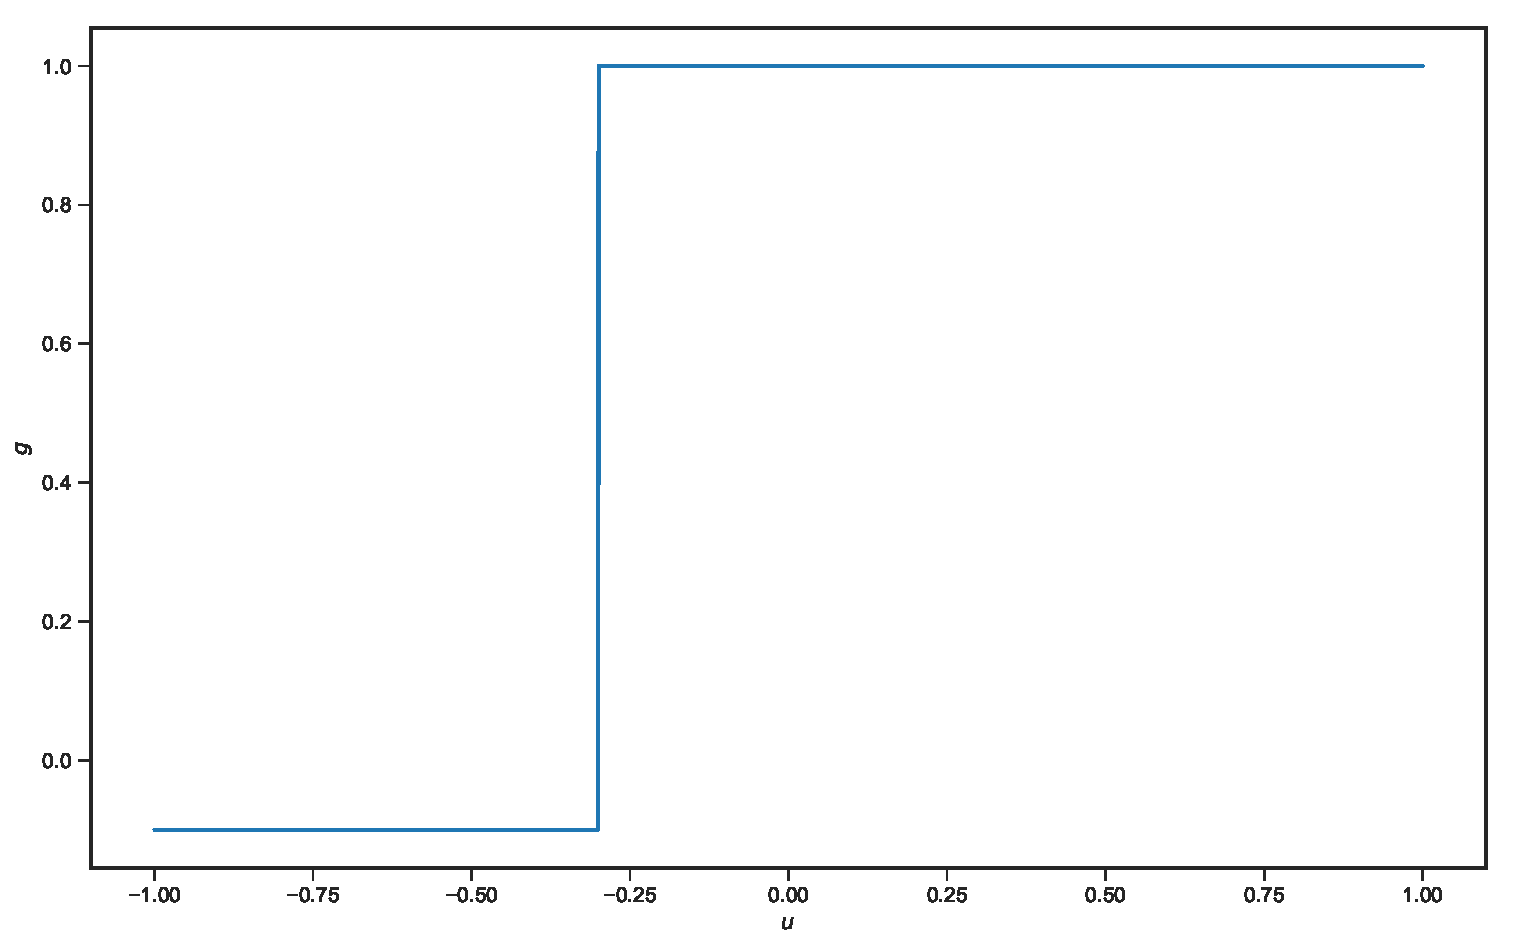
\includegraphics[width=\linewidth]{chapters/assets/dr/spectBoxC1Spectrum.pdf}
   % \endminipage\hfill
   \minipage{0.49\textwidth}
   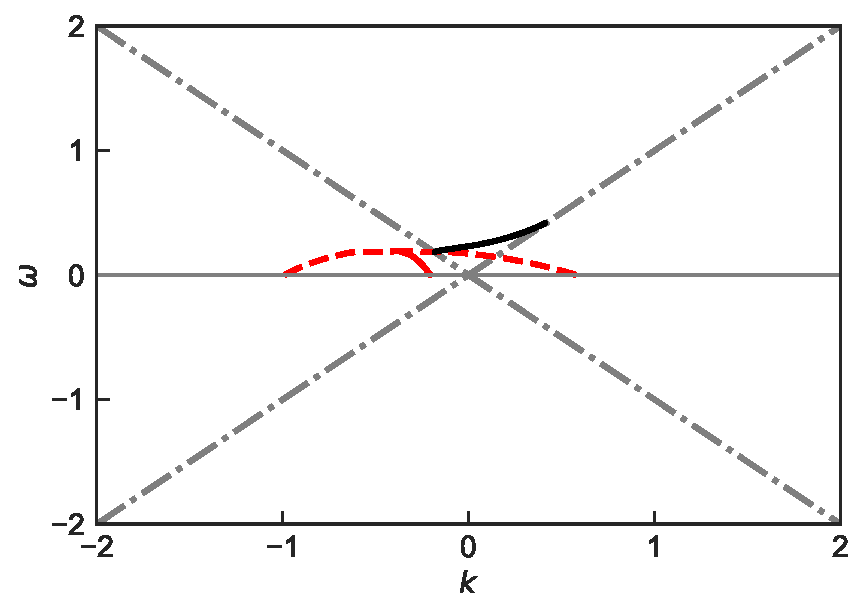
\includegraphics[width=\linewidth]{chapters/assets/dr/spectBoxC1MAADRPltBlob.pdf}
   \endminipage\hfill
   \minipage{0.49\textwidth}
   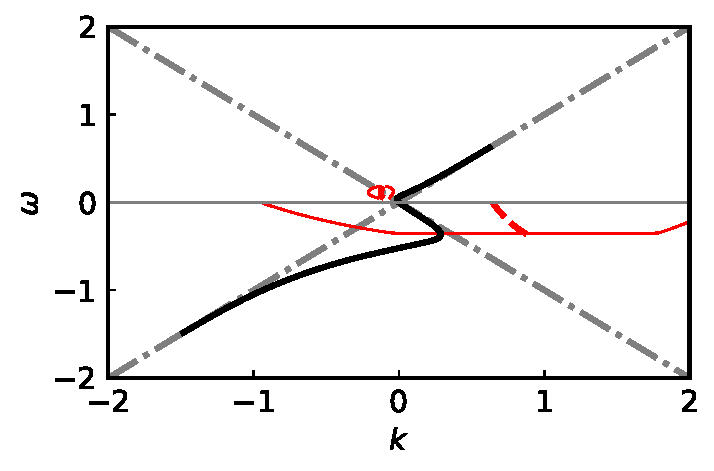
\includegraphics[width=\linewidth]{chapters/assets/dr/spectBoxC1MZADRPltBlob.pdf}
   \endminipage\hfill
   \caption{Dispersion relation and linear stability analysis for box spectrum. The box spectrum is defined to be $-0.1$ within range $u\in [-1,-0.3)$ and $1$ within range $u\in [-0.3,1]$. Left panel shows the dispersion relation and the complex $k$ for real $\omega$ for MAA solution. Right panel is the corresponding result for MZA solution. Dash-dotted gray lines are $\omega= \pm k$ which sets the boundaries of the forbidden region for dispersion relation.
    }
   \label{fig-box-c1}
\end{figure}





\section{\label{chap:dr-sec:conclusion}Conclusion}


We have reviewed that dispersion relation gap and instabilities are the same thing for neutrino emission with two zenith angles for the quadratic nature of the problem. As for more realistic spectrum, we have proved that instabilities propagate in regions of either $\omega>0$ or $\omega<0$ and never cross $\omega=0$. Hence the dispersion relation gaps should be defined as gaps between the dispersion relation curves and the axis $\omega=0$ instead of the dispersion relation curves. We have also showed that instabilities is not necessarily shown as gap in dispersion relations for neutrino emission with more than two zenith angles and box spectrum with crossing. Through the discussions, we demonstrated that the relation between dispersion relation gaps and instabilities should be used with caution.

